\chapter{Manipulação de Imagens em LaTeX}

\chapterquote{``Citação.''}{Autor}

% --------

\section{Introdução ao pacote \texttt{graphicx}}

O pacote \verb|graphicx| é essencial para inserir imagens. Carregue-o no pré-âmbulo:

\begin{lstlisting}[language=tex, caption=Carregue o pacote \texttt{graphicx}]
    \usepackage{graphicx} % Sempre adicione isso!
\end{lstlisting}

Formato de imagens suportados:
\begin{itemize}
    \item \textbf{Overleaf}: \verb|PNG|, \verb|JPG|, \verb|PDF| (evite \verb|SVG|, a menos que convertido.
    \item \textbf{LaTeX offline}: \verb|PDF|, \verb|EPS|, \verb|PNG|, \verb|JPG|
\end{itemize}

\section{Inserindo imagens básicas}

Use \verb|\includegraphics| para adicionar uma imagem:

\begin{lstlisting}[language=tex, caption=Inserindo uma imagem]
    \includegraphics[width=0.5\textwidth]{caminho/para/imagem.png}  
\end{lstlisting}

\section{Redimensionamento e escala}

\begin{itemize}
    \item Largura fixa: \verb|width=8cm|.
    \item Altura fixa: \verb|height=4cm|.
    \item Escala proporcional: \verb|scale=0.7|.
    \item Rotação: \verb|angle=45|
\end{itemize}

\begin{lstlisting}[language=tex, caption=Exemplo de customização do tamanho e ângulo de imagem]
    \includegraphics[width=5cm, angle=30]{imagem.jpg}  
\end{lstlisting}

\newpage

\section{Posicionamento com o ambiente \texttt{figure}}

O ambiente \verb|figure| permite controle profissional sobre posição, legendas e referências:

\begin{lstlisting}[language=tex, caption=Exemplo de customização do tamanho e ângulo de imagem]
    \begin{figure}[h!] % Opções: h (aqui), t (topo), b (base), p (página separada)
        \centering
        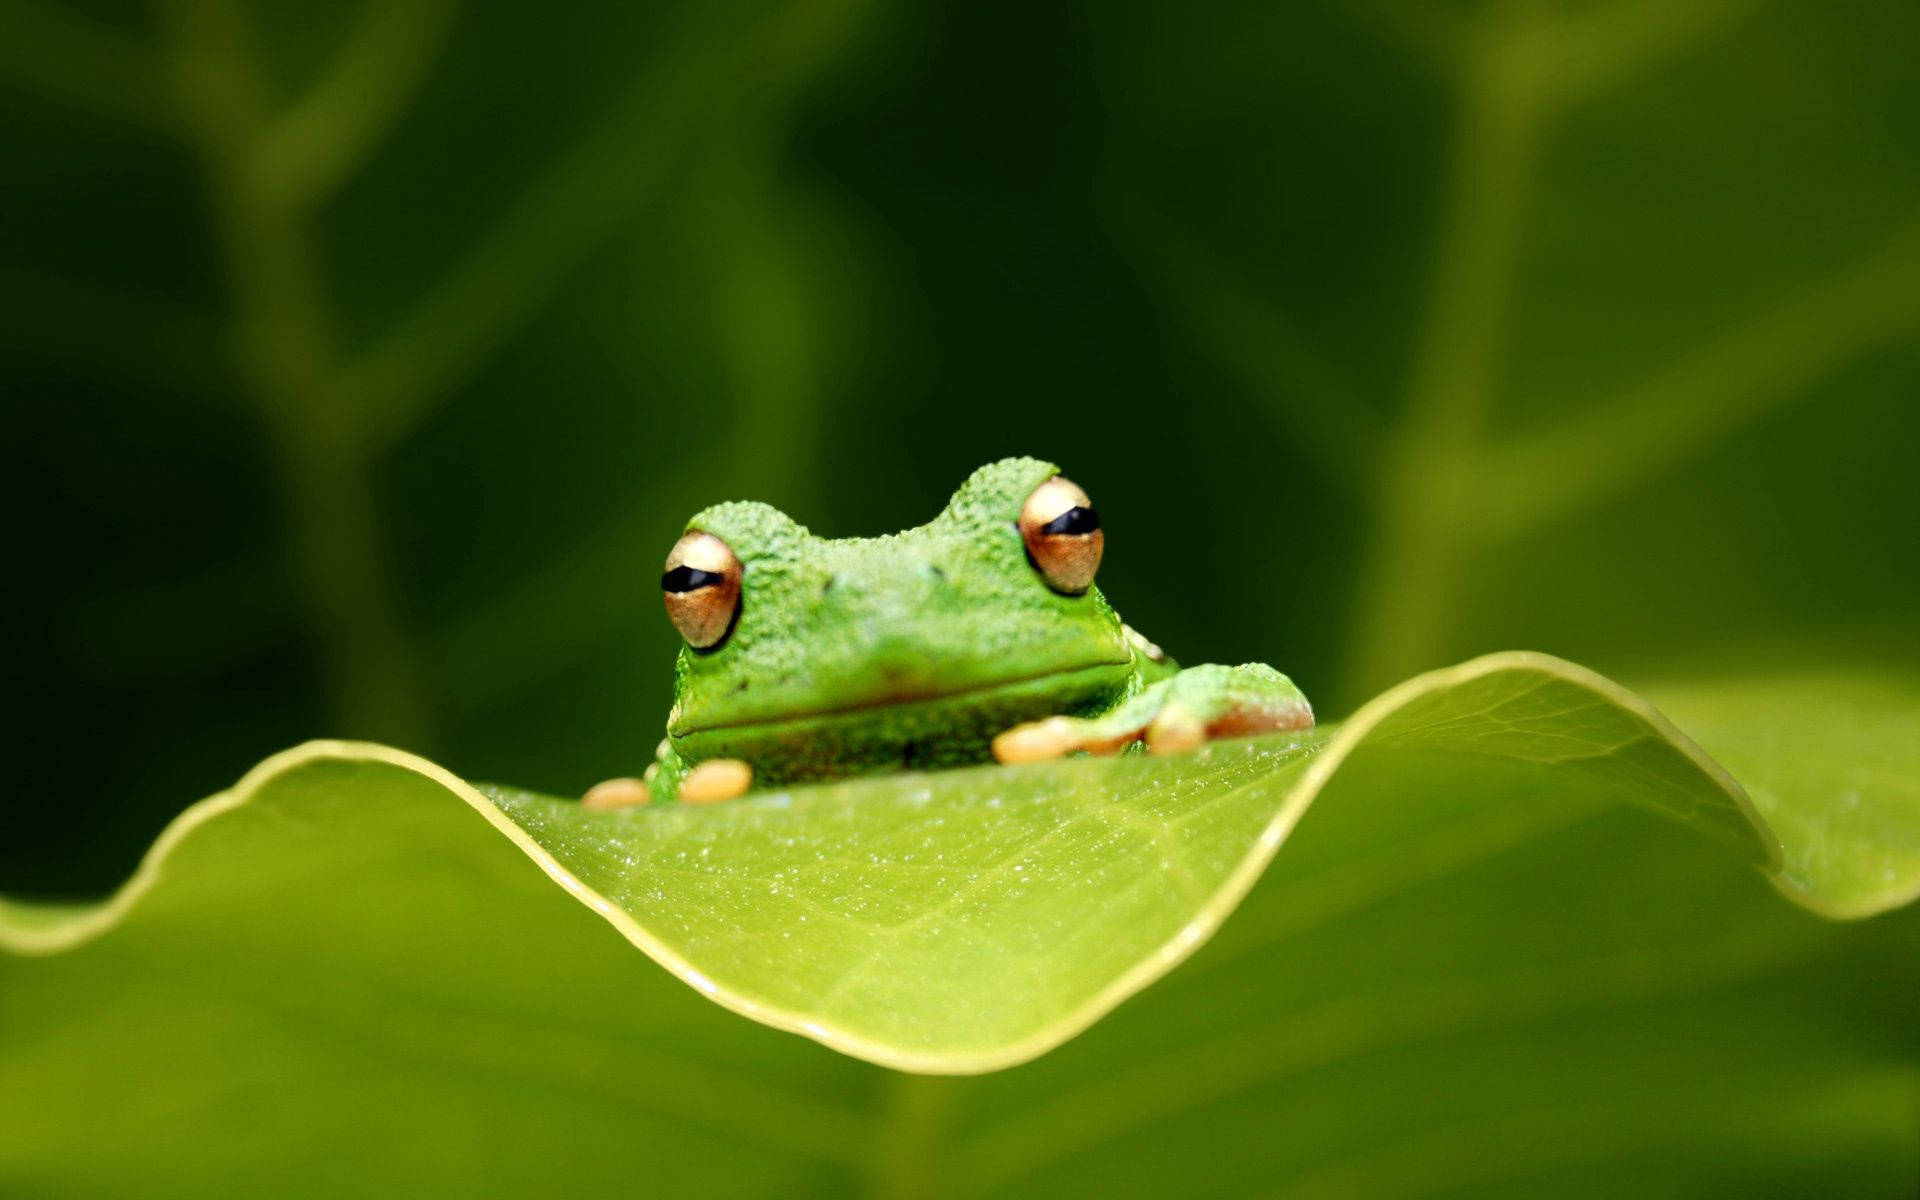
\includegraphics[width=0.4\textwidth]{imagens/sapo.jpg}
        \caption{Imagem da capa do livro} % Legenda
        \label{fig:sapodacapa} % Rótulo para referência
    \end{figure}
\end{lstlisting}

\begin{figure}[h!] % Opções: h (aqui), t (topo), b (base), p (página separada)
    \centering
    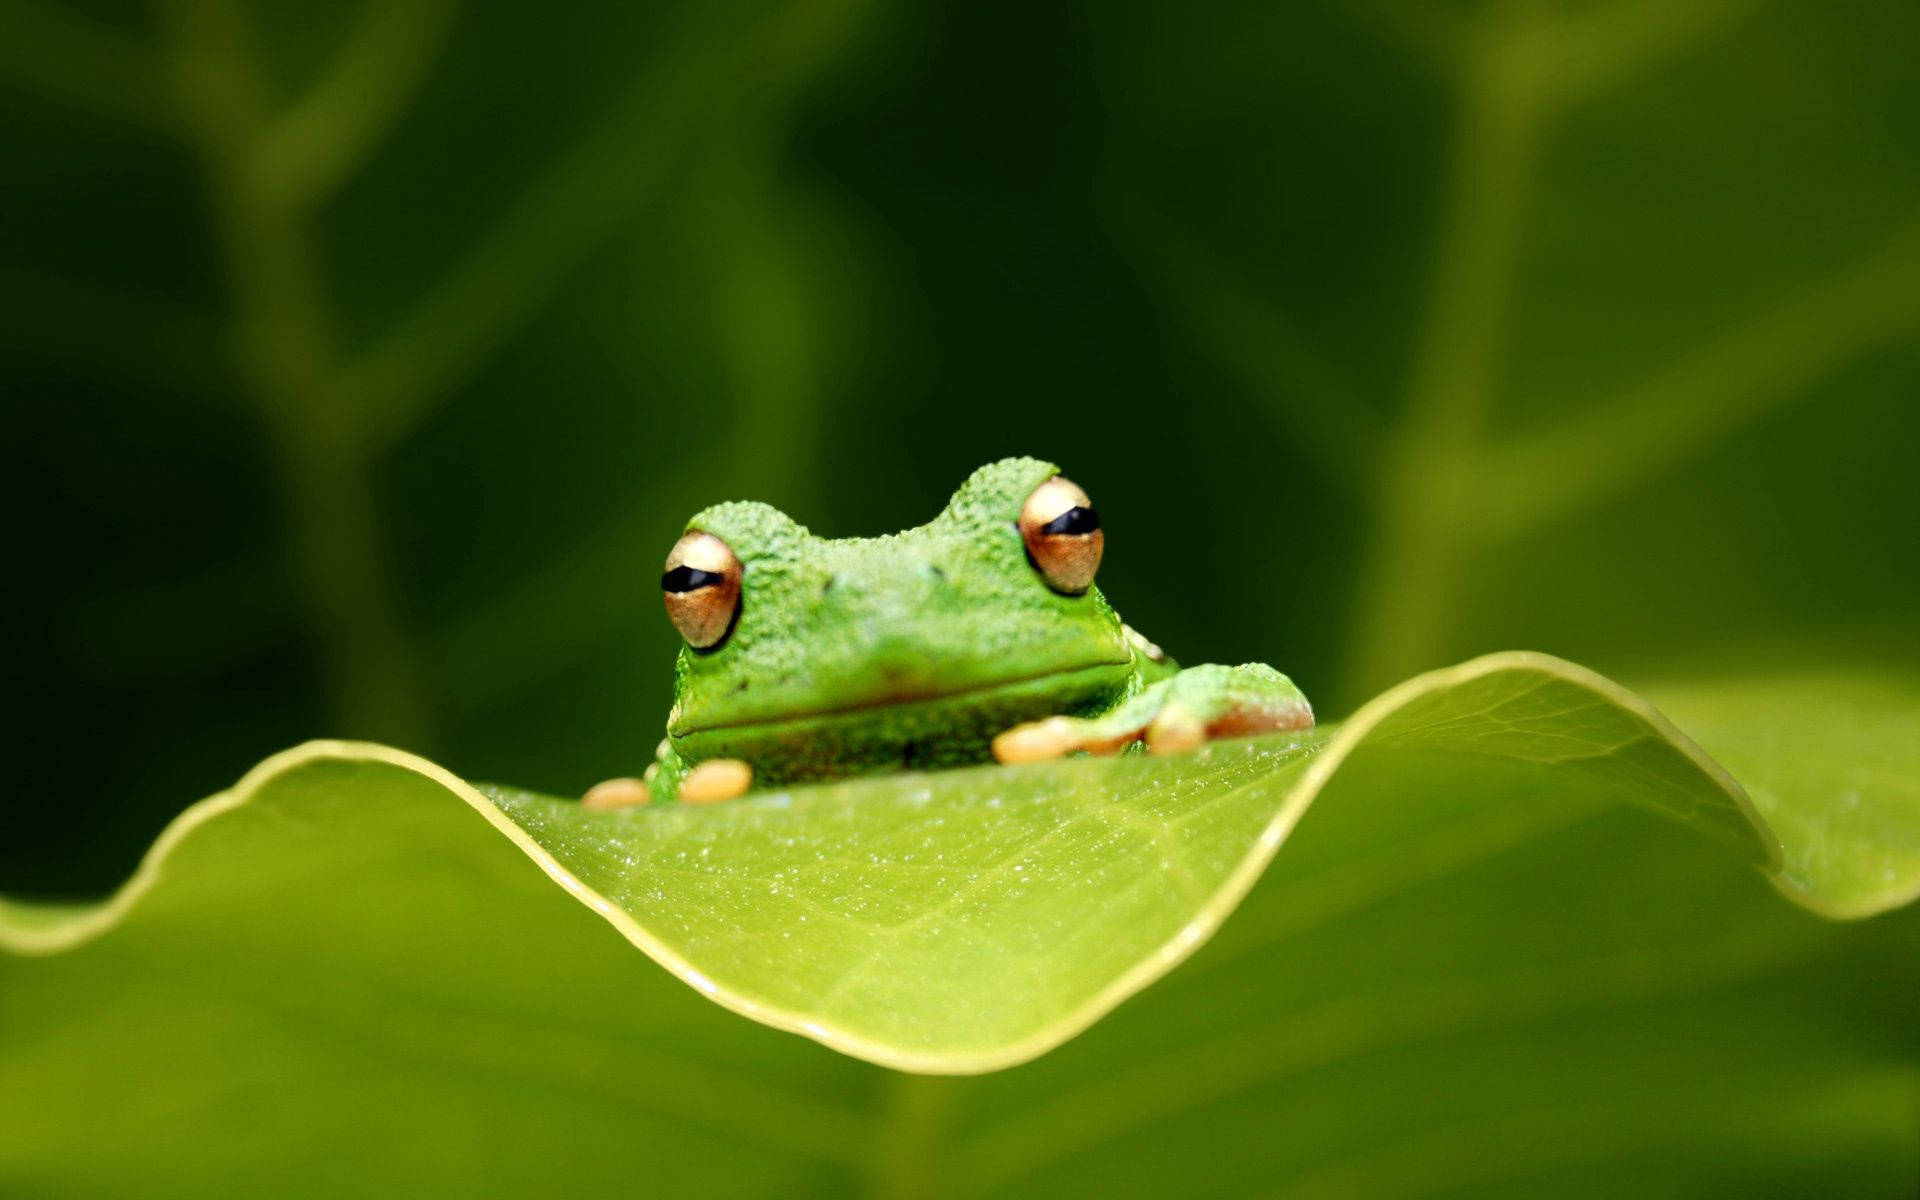
\includegraphics[width=0.7\textwidth]{imagens/sapo.jpg}
    \caption{Imagem da capa do livro} % Legenda
    \label{fig:sapodacapa} % Rótulo para referência
\end{figure}

\section{Múltiplas imagens em uma figura}

Use o pacote \verb|subcaption| para criar subfiguras:

\begin{lstlisting}[language=tex, caption=Exemplo de customização do tamanho e ângulo de imagem]
\begin{figure}[h]
    \centering
    \begin{subfigure}{0.45\textwidth}
        \includegraphics[width=\textwidth]{imagem1.jpg}
        \caption{Primeira imagem}
    \end{subfigure}
    \hfill
    \begin{subfigure}{0.45\textwidth}
        \includegraphics[width=\textwidth]{imagem2.jpg}
        \caption{Segunda imagem}
    \end{subfigure}
    \caption{Conjunto de imagens}
    \label{fig:duas-imagens}
\end{figure}
\end{lstlisting}

\begin{figure}[h]
    \centering
    \begin{subfigure}{0.45\textwidth}
        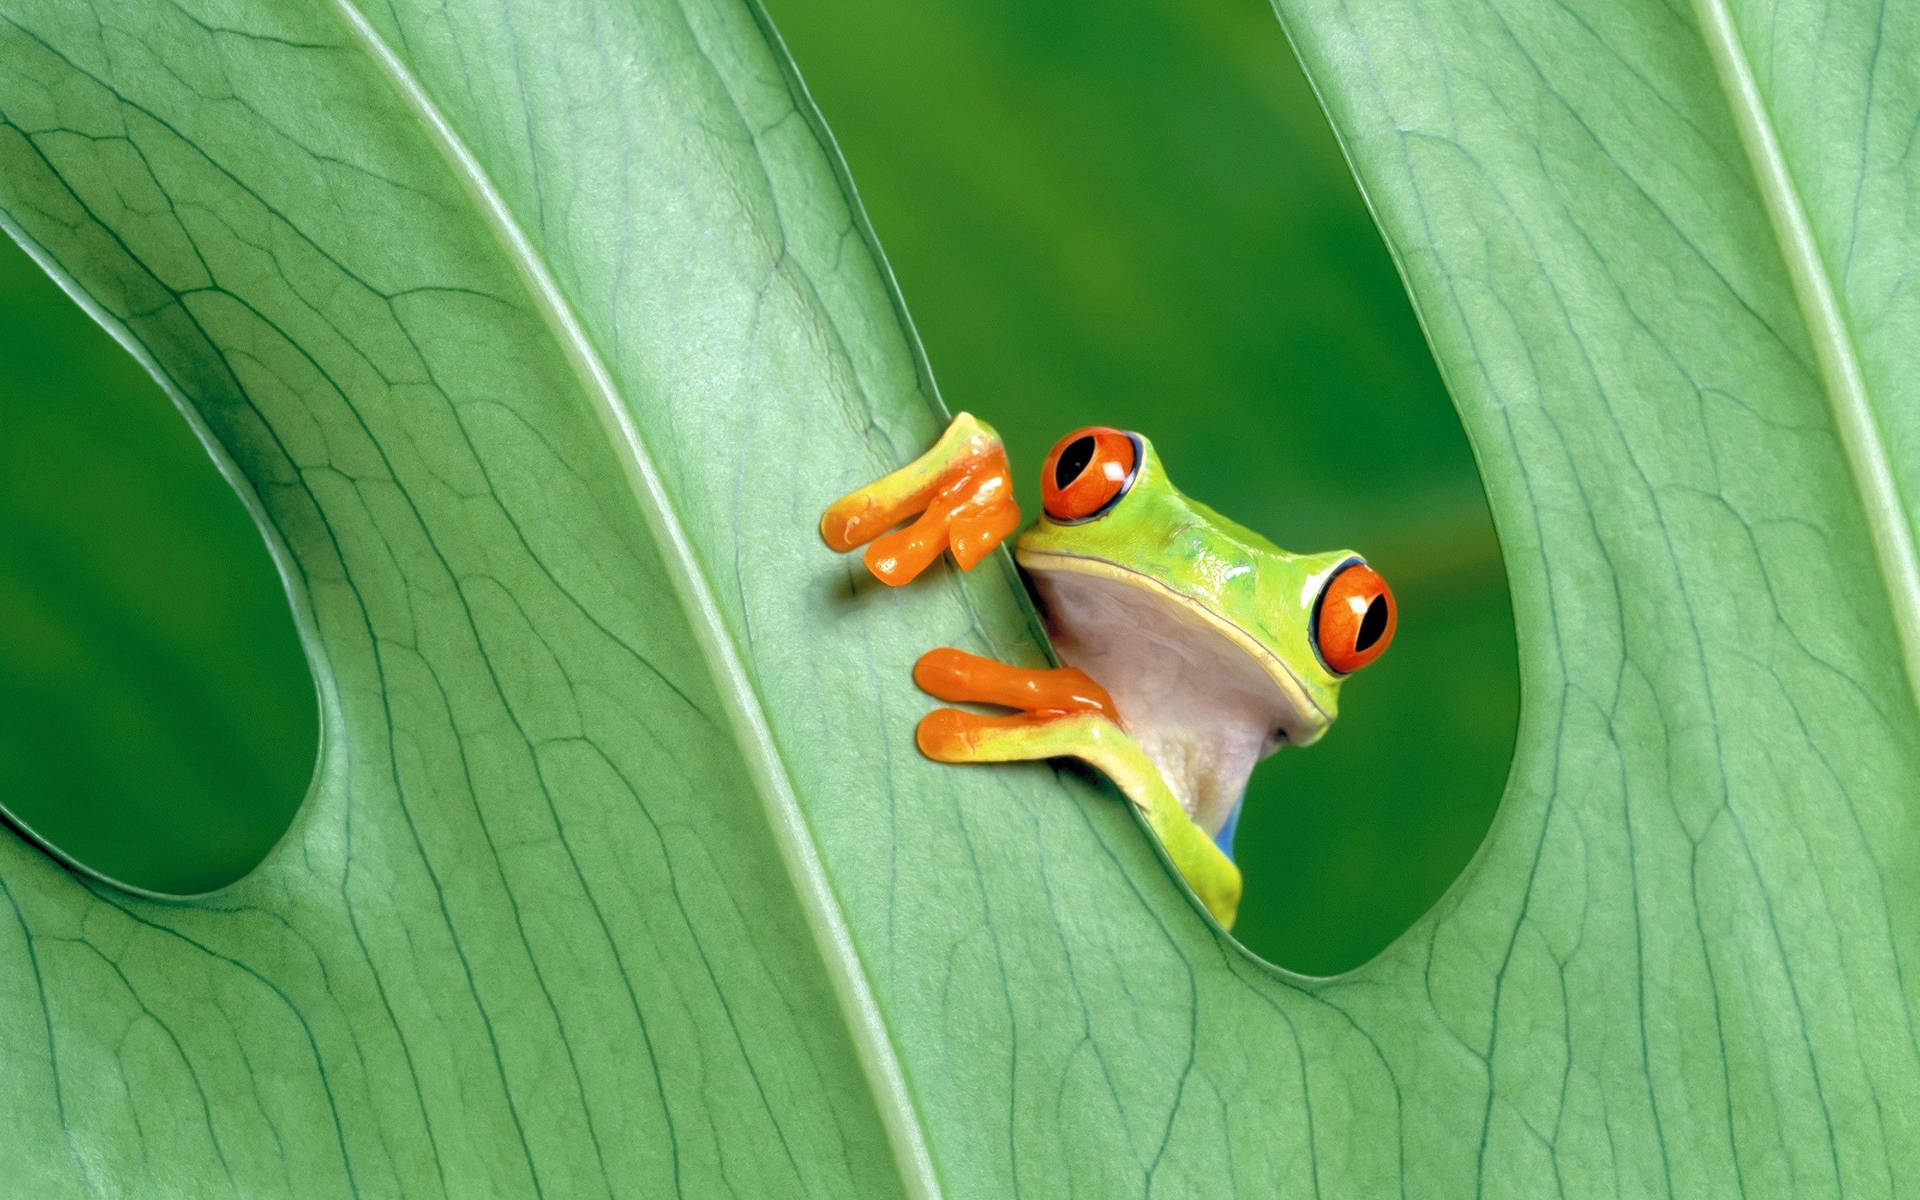
\includegraphics[width=\textwidth]{imagens/sapo1.jpg}
        \caption{Primeira imagem}
    \end{subfigure}
    \hfill
    \begin{subfigure}{0.45\textwidth}
        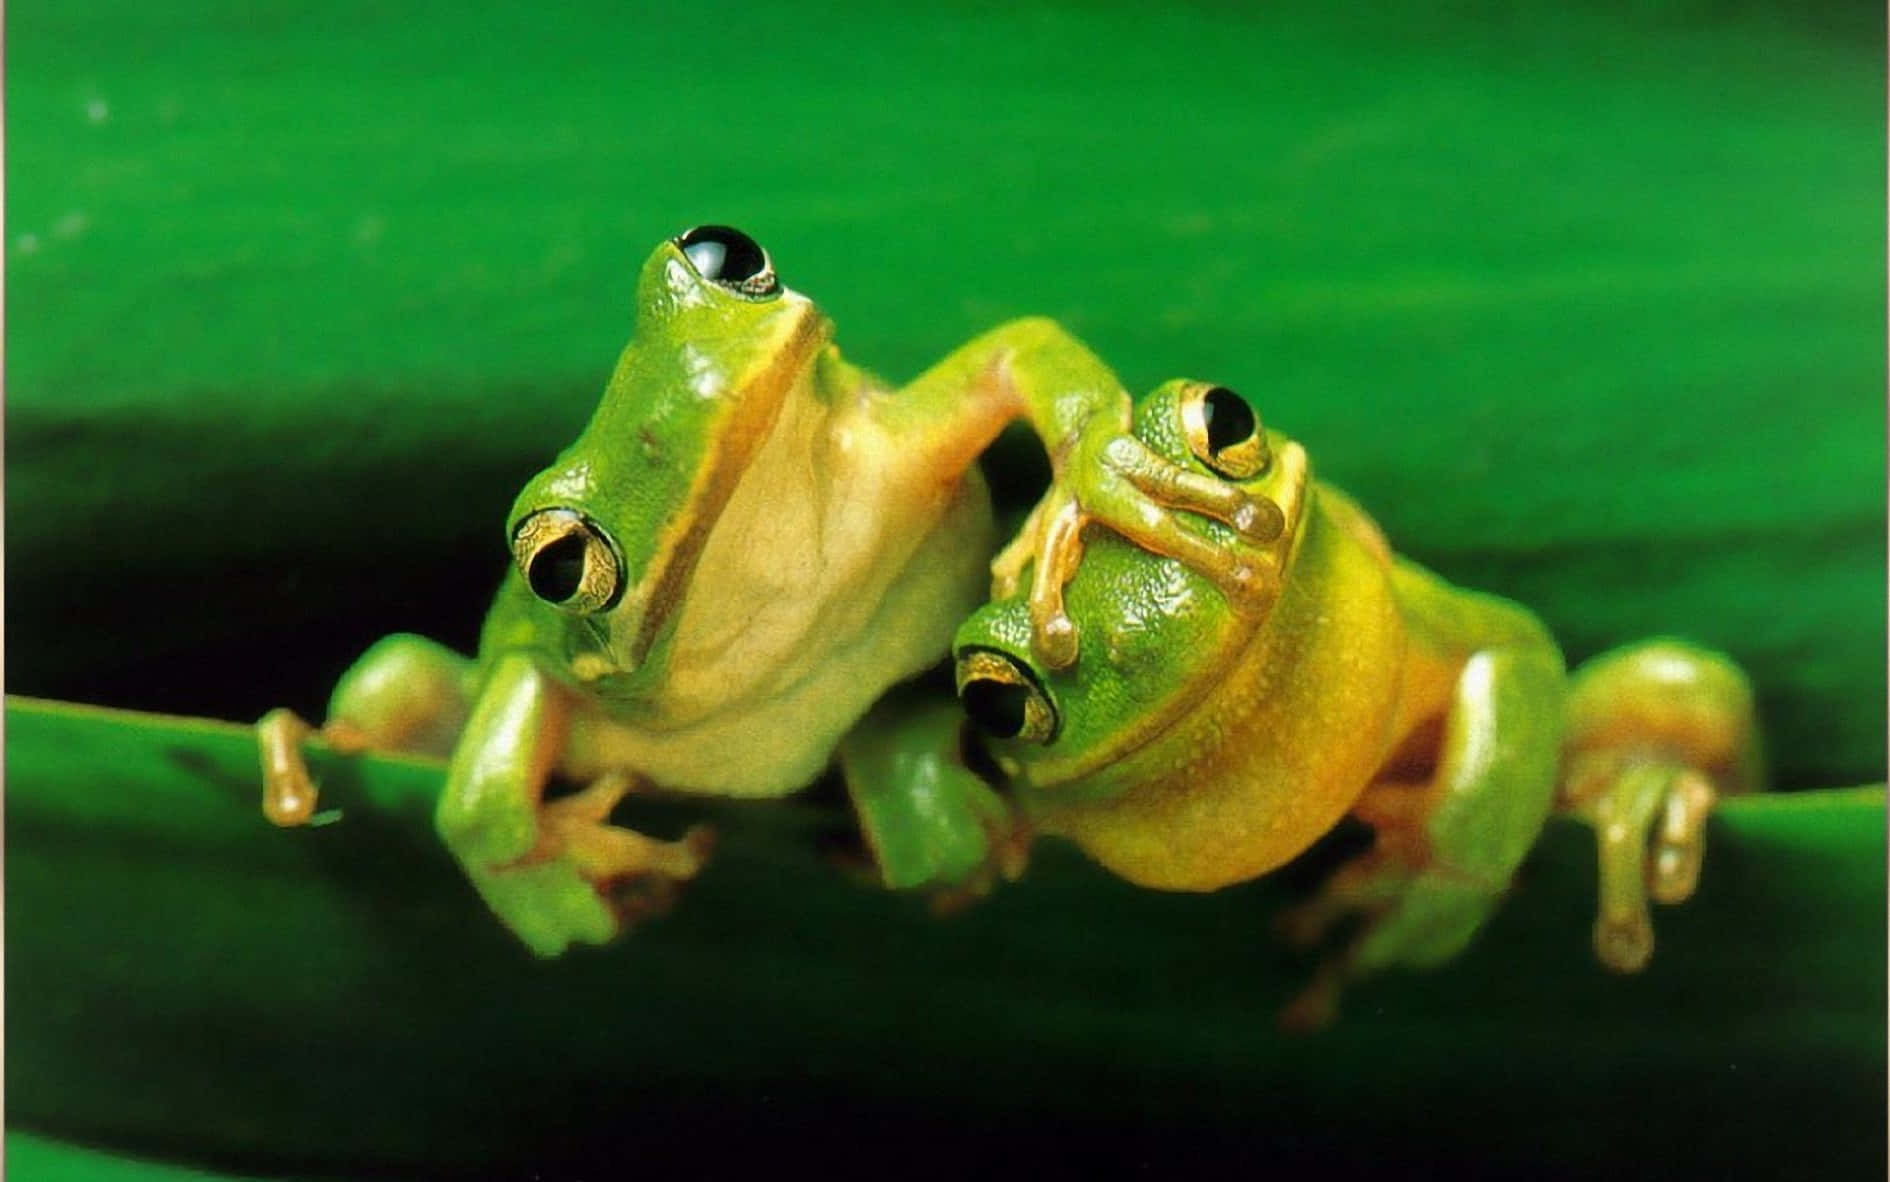
\includegraphics[width=\textwidth]{imagens/sapo2.jpg}
        \caption{Segunda imagem}
    \end{subfigure}
    \caption{Conjunto de imagens}
    \label{fig:duas-imagens}
\end{figure}

\section{Dicas práticas}
\begin{itemize}
    \item Armazene as imagens em uma pasta chamada \verb|imagens| e use:
    \begin{lstlisting}[language=tex, caption=Exemplo de customização do tamanho e ângulo de imagem]
    \graphicspath{{imagens/}} % Define o caminho padrão
    \includegraphics{logo} % Busca por "logo.png" ou "logo.jpg"
    \end{lstlisting}
    \item Erros comuns:
    \begin{itemize}
        \item Imagem não aparece: Verifique o caminho do arquivo e certifique que o pacote \verb|graphicx| está carregado.
        \item Legenda fora do lugar: Use \verb|\centering| dentro do ambiente \verb|figure|.
        \item Formato não suportado: Converta a imagem para um dos formatos suportados. 
    \end{itemize}
    
\end{itemize}
